\section{Introducción}
% Especificar la motivación y las características principales del proyecto como así también un marco general
% sobre el estado del arte de la tecnología y el uso de las ideas o conceptos del proyecto propuesto.
En el ámbito universitario resulta necesario mantener informadas a las personas sobre una amplia variedad de hechos, noticias y acontecimientos que sucedieron o sucederán, desde la ubicación de un aula hasta la notificación de la cancelación de una clase. Muchas veces estas notificaciones son sobre cuestiones muy efímeras, lo que requiere rapidez para empezar a transmitirlas y facilidad para tener el alcance necesario.

En las facultades de la Universidad Nacional de La Plata se consumen muchos recursos para cumplir este fin, a través de afiches, pancartas, panfletos, etc. los cuales, pese a ser de barata fabricación, no tienen una vida útil muy extensa. Además todas estas formas de comunicacion se basan en el uso de papel, que tras ser utilizado debe desecharse debido a la imposibilidad de reutilizarlo, generando una cantidad de residuos significativa. Si se tiene en cuenta que también generan una polución visual considerable, por la gran cantidad de estos distribuidos en todos los lugares transitables, resulta prudente considerar una nueva forma de comunicación.

Surge así la idea de desarrollar de un cartel electrónico reutilizable, capaz de ser configurado remotamente por las autoridades competentes, con el fin de proveer una forma de comunicación masiva más limpia, clara y menos dañina para el medio ambiente. 

\section{Objetivos del proyecto}
% Deben especificarse los objetivos que se plantearon en el informe inicial
% (primarios y secundarios) se hayan cumplido o no (en las conclusiones se deberá contemplar
% el cambio de objetivos o el grado de cumplimiento de los mismos).
El objetivo principal del proyecto es implementar un cartel de LEDs que pueda ser configurado remotamente por un usuario.
El mismo se puede subdividir en subobjetivos, los cuales se mencionan a continuación:

Diseñar e implementar el Hardware (PCB, matrices de LEDs) del cartel para que visualice correctamente el mensaje configurado. Deberá ser modularizable, es decir, que sea posible agregar módulos funcionales y expandir la cantidad de caracteres en un renglón.

Desarrollar el software embebido que se ejecutará en el microcontrolador.

Desarrollar el software que controla el cartel. Éste podrá ser usado desde una pc y tendrá una interfaz gráfica con formato de panel para controlar las características del mensaje a mostrar por el cartel.

Diseñar e implementar protocolo de comunicación para la comunicación entre el software controlador del panel y el cartel. El protocolo debe establecer un método de autenticación que impida el acceso de personal no autorizado al cartel. Esto implica que sea seguro antes ataque del tipo \emph{man-in-the-middle} y otros tipos de ataques bien conocidos.

\section{Análisis de requerimientos}
% Enumerar los requerimientos funcionales y  no funcionales sobre los que se diseñó la solución propuesta.
% Especificar los aspectos funcionales que el sistema deberá cumplir respecto del usuario y su interacción con el mismo.

\subsection{Funcionales}
\begin{itemize}
	\item La aplicación de escritorio deberá ser capaz de poder iniciar una conexión vía TLS con el sistema utilizando la misma para enviar los mensajes que el cliente desee. Además la aplicación será multiplataforma.
	\item La aplicación podrá enviar peticiones de forma de obtener el mensaje actual del cartel o incluso establecer uno nuevo. Por otra parte, también podrá pedir los datos de la red a la que el sistema estará conectado o cambiarlos.
	\item La aplicación deberá ser capaz de modificar características tales como parpadeo, velocidad de movimiento o estaticidad del mensaje.
	\item La aplicación permitirá al usuario, ingresar por teclado el mensaje que desea mostrar mediante los caracteres que se establecen en el estándar de codificación de caracteres ISO/IEC 8859-1 (ver \cite{CodifChar}).
	\item El sistema (cartel) deberá ser capaz de aceptar sólo conexiones por TLS\cite{TLS} de forma que las conexiones y el intercambio de paquetes sea cifrado y seguro.
	\item El cartel deberá poder procesar sólo mensajes a través del protocolo diseñado específicamente para este proyecto (ver Apéndice \ref{sec:protocolo})
	\item El cartel deberá mostrar los mensajes que desee el usuario.
	\item El cartel deberá poder almacenar y modificar sus credenciales de red de forma de poder conectarse al WiFi que el cliente desee.
	\item El cartel deberá persistir los datos de configuración y del mensaje que muestra, aún cuando el mismo haya sido desconectado de la red o de la energía.
\end{itemize}

\subsection{No funcionales}
\begin{itemize}
	\item El tiempo de desarrollo no debe ser mayor a seis semanas.
	\item El tiempo de respuesta del cartel no debe exceder los cinco segundos.
	\item La conexión debe estar cifrada para evitar intrusiones.
	\item El sistema entero no debe consumir mas de 30 Watts estando en operación normal.
\end{itemize}

\section{Diseño del hardware}
% Describir el hardware propuesto, comenzando por un diagrama en bloques, luego una descripción de las Interfaces eléctricas
% (conexiones poncho-EDU-CIAA) y de usuario (teclado, displays, etc)
% hasta llegar al detalle fino de los componentes y circuitos a utilizar y sus características.
El hardware está compuesto por módulos. Cada módulo es un dispositivo independiente que está armado con una matriz de LEDs de 8x8, un chip shifteador \cite{MAX7219} y componentes pasivos varios (ver figura \ref{fig:hw-moduloEsquematico}). 

Hay dos tipos de módulos: un maestro y un esclavo. El módulo maestro tiene adentro, además de lo listado anteriormente, un microcontrolador, regulador de tensión y un conector expuesto al usuario. Cada módulo esclavo no tiene un microcontrolador, y en cambio dos conectores en vez de uno, con la idea de que puedan conectarse varios esclavos en \emph{daisy-chain}, como se ilustra en la figura \ref{fig:esquema-general}.

Uno de los factores limitará la cantidad máxima de módulos esclavos que se pueden conectar será el amperaje máximo de la fuente de tensión y el regulador que se utilice en el módulo maestro.

\begin{figure}[ht!]
	\begin{center}
		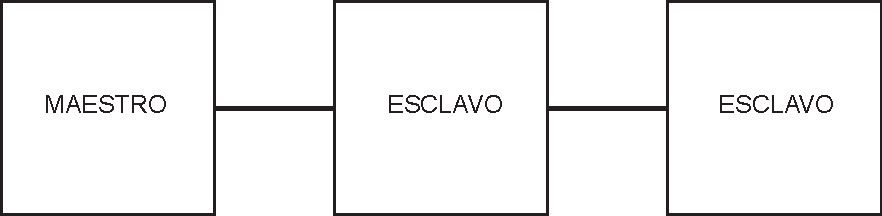
\includegraphics[scale=0.8]{imagenes/hw/esquema-general.pdf}
		\caption{Esquema general del sistema}
		\label{fig:esquema-general}
	\end{center}
\end{figure}

\subsection{Microcontrolador}
Como controlador principal se usará el kit de desarrollo NodeMCU, que integra un AI-Thinker ESP-12S, el cual contiene un SoC (\emph{System on Chip}) ESP8266EX de la empresa Espressif. El módulo NodeMCU es hardware libre, sin embargo, el resto de los componentes mencionados no lo son.\cite{NodeMCU}

El chip ESP8266EX combina un microcontrolador Tensillica Xtensa L106, un RISC de 32 bits corriendo a 80 Mhz, con funcionalidad WiFi. \cite{ESP8266Datasheet} El chip tiene memoria ROM con firmware no removible, y puede correr programas almacenados en flash externa. Para poder usar todas sus funcionalidades, se debe programar sobre firmware privativo desarrollado por Espressif, esto implica que el programa de usuario corre en simultáneo con el firmware y el uso de la memoria de trabajo está sujeto a la versión del firmware. Según el datasheet, el usuario puede esperar tener disponible 50 KiB de SRAM.

Como se mencionó anteriormente, se necesita de flash externa para correr programas. El módulo ESP-12S se encarga de proveer al ESP8266EX 4MiB de memoria flash.

\subsection{Módulos}
El cartel se compone de módulos: un maestro y esclavos. Cada módulo contiene una matriz de LED 8x8, un chip shifteador \cite{MAX7219} y componentes pasivos varios (ver figura \ref{fig:hw-moduloEsquematico}). A diferencia de un modulo esclavo, el maestro posee un microcontrolador NodeMCU que recibe los pedidos del usuario, procesa la información codificando los caracteres y transmite a los esclavos conectados que muestren la información.

\begin{figure}[ht!]
	\begin{center}
		\includegraphics[width=0.8\textwidth]{imagenes/hw/moduloEsquematico}
		\caption{Esquema de conexiones de un módulo funcional.}
		\label{fig:hw-moduloEsquematico}
	\end{center}
\end{figure}


\begin{figure}[ht!]
	\begin{center}
		\includegraphics[width=0.7\textwidth]{imagenes/hw/moduloLED}
		\caption{Esquema de conexiones de un módulo funcional.}
		\label{fig:hw-moduloLED}
	\end{center}
\end{figure}

El MAX7219 recibe una secuencia de bytes por serie y los deriva a la columna que corresponda para cada instante en la matriz de LEDs del módulo correspondiente en el cartel. 

\section{Diseño de software}
% Descripción del software propuesto, comenzando por un diagrama de estados, pseudocódigo o esquemas que permitan
% comprender la arquitectura de software elegida (Controlada por eventos o por tiempo, apropiativa, cooperativa, etc).
% Luego especificar las diferentes módulos (o tareas) a implementar, drivers, bibliotecas a utilizar,
% prioridades y planificación de las distintas tareas (No incluir en el informe código C).
El sistema a nivel software consiste de la aplicación de escritorio que va a controlar el cartel y el software que corre en el microcontrolador.
La comunicación de estas dos componentes se hará a través de una red IP. El cartel estará asociado a una red WiFi, lo cual le permitirá aceptar conexiones provinientes de hosts locales a la red o incluso externos a la red dado que está provisto el ruteo adecuado. 

El protocolo a utilizarse es un protocolo binario personalizado específico a esta aplicación. Para brindar seguridad y autenticación, toda transmisión se hara sobre una conexión segura TLS. 

El protocolo está especificado en detalle en el Apéndice \ref{sec:protocolo}.


\subsection{Panel de configuración}
El panel de configuración consiste en una aplicación multiplataforma de escritorio escrita en C++ utilizando el framework de desarrollo Qt, que tiene como objetivo conectarse con el módulo NodeMCU (ESP8266) presente en el cartel a través de una conexión TLS.

La aplicación inicia la conexión con el sistema y, una vez establecida, permite cambiar el mensaje a mostrar, recuperar el mensaje completo que se está mostrando actualmente, cambiar opciones de animación, y modificar la red a la cual el cartel se conectará la próxima vez que se reinicie.

En la figura \ref{fig:screenshot-panel} se observa una captura de pantalla de la aplicación de escritorio.

\begin{figure}[ht!]
	\begin{center}
		\centering
		\includegraphics[scale=0.8]{imagenes/screenshot-panel.png}
		\caption{Captura de pantalla de la aplicación de escritorio.}
		\label{fig:screenshot-panel}
	\end{center}
\end{figure}

\subsection{Software embebido}
El software que corre en el microcontrolador del cartel debe escuchar conexiones TLS, y una vez establecida una conexión iniciada por la aplicación de escritorio, debe esperar a recibir un mensaje de autenticación antes de permitir cambios del mensaje.

Una vez que el usuario se autentica, el cartel espera un pedido de la aplicación de escritorio. Las interacciones posibles están descritas en el apéndice \ref{sec:protocolo}.

El comportamiento del microcontrolador del cartel puede describirse como una máquina de estado finita jerárquica, como lo muestra la figura \ref{fig:fsm-micro}.

\begin{figure}[ht!]
	\begin{center}
		\centering
		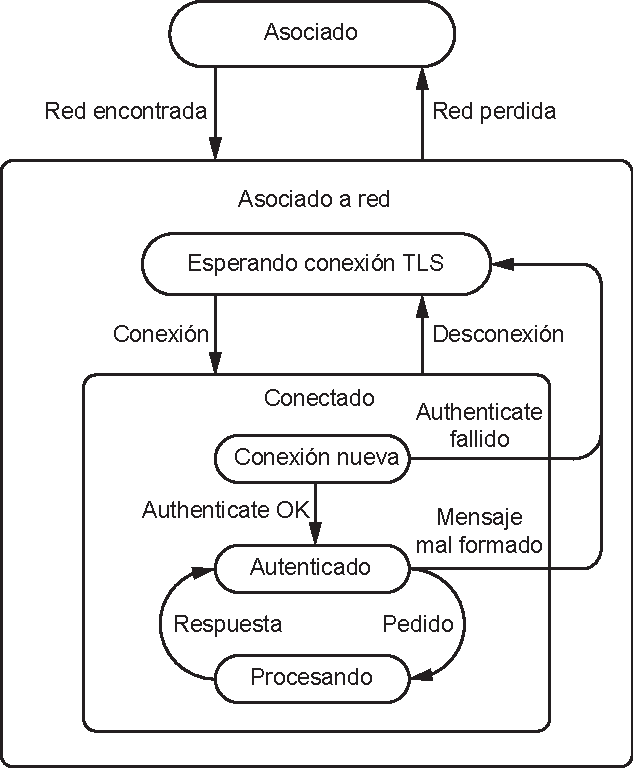
\includegraphics[scale=0.8]{imagenes/fsm-micro.pdf}
		\caption{Máquina de estados finitos jerárquica del manejo de conexión en el microcontrolador.}
		\label{fig:fsm-micro}
	\end{center}
\end{figure}

El ESP8266 se puede programar utilizando el SDK de la empresa que desarrolló el chip, Espressif. Existen dos versiones del SDK, una basada en FreeRTOS, lo cual permite tener tareas en ejecución simultánea, y otra que no está basada en tareas, sino que todo el código del usuario consiste en callbacks que se ejecutan de forma cooperativa y deben retornar rápidamente.

Se decidió utilizar la versión basada en callbacks ya que elimina muchos problemas de programación concurrente al asegurar que las funciones siempre se ejecutan de forma aparentemente atómica. (salvo posiblemente por interrupciones que el firmware utiliza internamente)

\subsubsection{Almacenamiento de los caracteres}
\begin{figure}[h!]
    \centering
    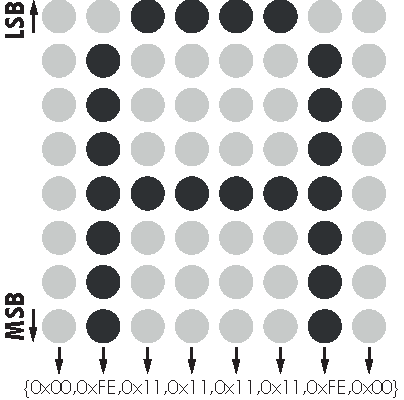
\includegraphics[width=0.47\textwidth]{imagenes/codificacionAscii.pdf}
    \caption{Representación de los caracteres en el cartel.}
    \label{fig:repAscii}
\end{figure}


Los caracteres que son recibidos en el microcontrolador son codificados en mapa de bits, en el que un bit representa el estado (encendido o apagado) de un LED en particular según la posición en el que esté, para poder representarlos correctamente en la matriz. En la figura \ref{fig:repAscii} se observa un ejemplo de como esta representada la letra \enquote{A} en el mapa de bits.

Cada byte corresponde a una columna del carácter a mostrar y a su vez el LED inferior se codifica como el más significativo (MSB) y el superior se codifica como el menos significativo (LSB). De esta forma se envía al MAX7219 ocho bytes por cada carácter que se desea mostrar en la matriz.

Por otro lado, respetando el orden en que se establecen los caracteres el estándar ISO/IEC 8859-1, se guardan en un archivo los ocho bytes de cada carácter.

\section{Ensayos y mediciones}
% Describir el proceso de construcción del prototipo y los ensayos realizados para verificar el funcionamiento del mismo.
% Mostrar mediciones o resultados obtenidos en forma de tablas, figuras, 
% fotografías del sistema, pantallas de osciloscopios, pantallas de display, etc
Se desarrolló un prototipo de uno de los módulos funcionales del cartel, conectando los componentes sobre una protoboard y soldando una matriz de LEDs con la disposición a utilizar en el modelo final (ver Figura \ref{fig:hw-moduloLED}).

A través del mismo se hicieron pruebas para corroborar el correcto funcionamiento particular de un módulo funcional y la claridad del carácter mostrado. Se corroboró que el mensaje comienza a mostrarse pocos instantes después de que el mismo empieza a ser recibido por el cartel.

También se puso a prueba la tensión máxima soportada por los LEDs utilizados, los cuales demostraron la capacidad de soportar hasta 4,2 V de tensión con una corriente continua de 20 mA. En dicho prototipo se usaron resistencias que diferían levemente de las planteadas en el esquema original debido a problemas de disponibilidad de las mismas, confirmando que el módulo funciona correctamente con un margen de tolerancia para los valores de tensión y corriente en los LEDs.

El prototipo también permitió confirmar que el sistema puede prescindir de un disipador térmico ya que los componentes no levantan una temperatura considerable, aún después de un funcionamiento prolongado.


\section{Conclusiones parciales}
% 1-Explicar el grado de avance de los objetivos planteados hasta el momento como así también el trabajo a seguir.
% 2-Describir claramente la actividad de cada integrante del grupo, evaluar las horas invertidas hasta el momento
%	y re-estimar las horas de ingeniería restantes.
% 3- Evaluar y destacar correcciones o desvíos del cronograma de tareas presentado en el informe de inicial.
% 4-Analizar el presupuesto invertido y corregir (si corresponde) el presupuesto final del proyecto. 

Ternouski y Levy plantearon el esquema de hardware y desarrollaron el primer prototipo del módulo funcional. La duración de la tarea estipulada fue de dos días y la duración real de casi dos días.

Ternouski y Levy corroboraron que la implementación práctica de la matriz de LEDs usando el esquema planteado originalmente permite mostrar correctamente el mensaje que el usuario disponga. La duración estimada fue de un día y se cumplió satisfactoriamente.

Romero y García diseñaron un protocolo para la comunicación entre el panel de configuración y el cartel (ver Apéndice \ref{sec:protocolo}). La duración de la tarea cumplió con el tiempo estimado de tres días.

Romero y García redactaron un primer borrador relacionado a la especificación del protocolo diseñado. La duración de la tarea cumplió con el tiempo estimado de dos días.

Ternouski y Romero desarrollaron la interfaz gráfica de la aplicación de escritorio a utilizar para que el usuario configure el mensaje junto con otro programa que simula una matriz de 8x8 y permite al usuario diseñar los caracteres a mano. Se puede ver una captura de pantalla de la aplicación de escritorio en la figura \ref{fig:screenshot-panel}. La duración de la tarea cumplió con el tiempo calculado de tres días.

Romero y García escribieron un programa base en el módulo ESP8266 que acepta conexiones TLS y, a modo de prueba, se programó para que envíe periódicamente mensajes de prueba a quién se conecte. La duración de la tarea cumplió con el tiempo estimado de cinco días.

Ternouski y Romero desarrollaron una aplicación de escritorio, que consiste en un cliente QT, con el objetivo de probar las conexiones TLS que se utilizarán para el intercambio de información entre el usuario y el sistema. La duración de la tarea cumplió con el tiempo calculado de cuatro días.

\subsection{Cronograma}
Como se puede observar en el apartado de las conclusiones parciales, el desarrollo de las actividades viene cumpliendo satisfactoriamente con los tiempos del cronograma estipulado. En el cronograma presente en la figura se observa las actividades que quedan realizar. En principio no se realizará ninguna corrección en cuanto al tiempo estipulado de las tareas que quedan por completar.


%TODO poner cronograma.

\subsection{Presupuesto}
%TODO: expandir
Hasta el momento el presupuesto invertido por los alumnos en el proyecto para el desarrollo del prototipo de un módulo funcional ronda los 500 pesos.